\documentclass[aspectratio=169]{beamer}
\usetheme{Madrid}
\usepackage[utf8]{inputenc}
\usepackage{amsmath}
\usepackage{amssymb}
\usepackage{tikz}
\usepackage{pgfplots}
\pgfplotsset{compat=1.17}

\title{Higher-Order Derivatives, Taylor's Theorem, and Convexity}
\author{}
\date{}

\begin{document}

\begin{frame}
\titlepage
\end{frame}

\begin{frame}{Outline}
\tableofcontents
\end{frame}

\section{Higher-Order Derivatives}

\begin{frame}{Definition of Higher-Order Derivatives}
\textbf{First Derivative:} $f'(x) = \lim_{h \to 0} \frac{f(x+h) - f(x)}{h}$

\vspace{0.5cm}

\textbf{Second Derivative:} The derivative of the first derivative
$$f''(x) = \frac{d}{dx}[f'(x)]$$

\vspace{0.5cm}

\textbf{Third Derivative:} $f'''(x) = \frac{d}{dx}[f''(x)]$

\vspace{0.5cm}

\textbf{$n$-th Derivative:} $f^{(n)}(x)$ denotes the $n$-th derivative

\vspace{0.3cm}
\textbf{Notation:}
$$f'(x), \quad f''(x), \quad f'''(x), \quad f^{(4)}(x), \ldots, \quad f^{(n)}(x)$$
or
$$\frac{df}{dx}, \quad \frac{d^2f}{dx^2}, \quad \frac{d^3f}{dx^3}, \quad \ldots, \quad \frac{d^nf}{dx^n}$$
\end{frame}

\begin{frame}{Examples of Higher-Order Derivatives}
\textbf{Example 1:} $f(x) = x^4$
\begin{align*}
f'(x) &= 4x^3 \\
f''(x) &= 12x^2 \\
f'''(x) &= 24x \\
f^{(4)}(x) &= 24 \\
f^{(5)}(x) &= 0
\end{align*}

\textbf{Example 2:} $f(x) = e^x$
$$f'(x) = f''(x) = f'''(x) = \cdots = f^{(n)}(x) = e^x$$
\end{frame}

\begin{frame}{Examples of Higher-Order Derivatives (Continued)}
\textbf{Example 3:} $f(x) = \sin(x)$
\begin{align*}
f'(x) &= \cos(x) \\
f''(x) &= -\sin(x) \\
f'''(x) &= -\cos(x) \\
f^{(4)}(x) &= \sin(x)
\end{align*}
The pattern repeats every 4 derivatives.

\vspace{0.5cm}

\textbf{Example 4:} $f(x) = \ln(x)$
\begin{align*}
f'(x) &= \frac{1}{x} \\
f''(x) &= -\frac{1}{x^2} \\
f'''(x) &= \frac{2}{x^3} \\
f^{(n)}(x) &= \frac{(-1)^{n+1}(n-1)!}{x^n}
\end{align*}
\end{frame}

\begin{frame}{Visualizing Higher-Order Derivatives}
\begin{center}
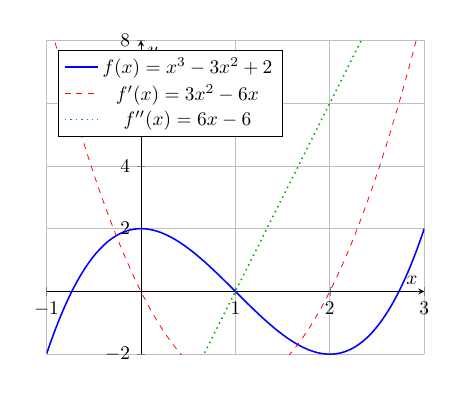
\begin{tikzpicture}[scale=0.7]
\begin{axis}[
    axis lines=middle,
    xlabel={$x$},
    ylabel={$y$},
    domain=-1:3,
    samples=100,
    grid=major,
    legend pos=north west,
    ymin=-2, ymax=8
]
\addplot[blue, thick] {x^3 - 3*x^2 + 2};
\addlegendentry{$f(x) = x^3 - 3x^2 + 2$}

\addplot[red, dashed] {3*x^2 - 6*x};
\addlegendentry{$f'(x) = 3x^2 - 6x$}

\addplot[green!70!black, dotted, thick] {6*x - 6};
\addlegendentry{$f''(x) = 6x - 6$}
\end{axis}
\end{tikzpicture}
\end{center}
The second derivative $f''(x)$ tells us about the curvature of $f(x)$.
\end{frame}

\begin{frame}{Physical Interpretation}
If $s(t)$ represents position at time $t$:

\vspace{0.5cm}

\textbf{First Derivative:} $s'(t) = v(t)$ is \textit{velocity}
$$v(t) = \frac{ds}{dt}$$

\vspace{0.5cm}

\textbf{Second Derivative:} $s''(t) = v'(t) = a(t)$ is \textit{acceleration}
$$a(t) = \frac{dv}{dt} = \frac{d^2s}{dt^2}$$

\vspace{0.5cm}

\textbf{Third Derivative:} $s'''(t) = a'(t)$ is \textit{jerk} (rate of change of acceleration)
$$j(t) = \frac{da}{dt} = \frac{d^3s}{dt^3}$$
\end{frame}

\section{Taylor's Theorem}

\begin{frame}{Motivation for Taylor Series}
\textbf{Question:} Can we approximate a complicated function with a polynomial?

\vspace{0.5cm}

\textbf{Linear Approximation:} Near $x = a$:
$$f(x) \approx f(a) + f'(a)(x-a)$$

\vspace{0.3cm}
This is the tangent line approximation.

\vspace{0.5cm}

\textbf{Quadratic Approximation:} Include curvature:
$$f(x) \approx f(a) + f'(a)(x-a) + \frac{f''(a)}{2}(x-a)^2$$

\vspace{0.5cm}

\textbf{Taylor's Theorem} extends this idea to higher-order approximations.
\end{frame}

\begin{frame}{Taylor's Theorem}
\textbf{Taylor Polynomial of degree $n$ at $x = a$:}
$$P_n(x) = f(a) + f'(a)(x-a) + \frac{f''(a)}{2!}(x-a)^2 + \cdots + \frac{f^{(n)}(a)}{n!}(x-a)^n$$

\vspace{0.3cm}

or more compactly:
$$P_n(x) = \sum_{k=0}^{n} \frac{f^{(k)}(a)}{k!}(x-a)^k$$

\vspace{0.5cm}

\textbf{Taylor Series:} If the limit exists as $n \to \infty$:
$$f(x) = \sum_{k=0}^{\infty} \frac{f^{(k)}(a)}{k!}(x-a)^k$$

\vspace{0.5cm}

\textbf{Maclaurin Series:} Special case when $a = 0$:
$$f(x) = \sum_{k=0}^{\infty} \frac{f^{(k)}(0)}{k!}x^k$$
\end{frame}

\begin{frame}{Common Taylor Series (Maclaurin Series)}
\textbf{Exponential:}
$$e^x = 1 + x + \frac{x^2}{2!} + \frac{x^3}{3!} + \cdots = \sum_{k=0}^{\infty} \frac{x^k}{k!}$$

\vspace{0.3cm}

\textbf{Sine:}
$$\sin(x) = x - \frac{x^3}{3!} + \frac{x^5}{5!} - \frac{x^7}{7!} + \cdots = \sum_{k=0}^{\infty} \frac{(-1)^k x^{2k+1}}{(2k+1)!}$$

\vspace{0.3cm}

\textbf{Cosine:}
$$\cos(x) = 1 - \frac{x^2}{2!} + \frac{x^4}{4!} - \frac{x^6}{6!} + \cdots = \sum_{k=0}^{\infty} \frac{(-1)^k x^{2k}}{(2k)!}$$

\vspace{0.3cm}

\textbf{Natural Logarithm:}
$$\ln(1+x) = x - \frac{x^2}{2} + \frac{x^3}{3} - \frac{x^4}{4} + \cdots = \sum_{k=1}^{\infty} \frac{(-1)^{k+1} x^k}{k}, \quad |x| < 1$$
\end{frame}

\begin{frame}{Example: Taylor Series for $e^x$}
\textbf{Find the Maclaurin series for $f(x) = e^x$:}

\vspace{0.3cm}

All derivatives of $e^x$ equal $e^x$, so:
\begin{align*}
f(0) &= e^0 = 1 \\
f'(0) &= e^0 = 1 \\
f''(0) &= e^0 = 1 \\
&\vdots \\
f^{(n)}(0) &= 1
\end{align*}

\vspace{0.3cm}

Therefore:
$$e^x = 1 + x + \frac{x^2}{2!} + \frac{x^3}{3!} + \frac{x^4}{4!} + \cdots$$
\end{frame}

\begin{frame}{Visualizing Taylor Approximations}
\begin{center}
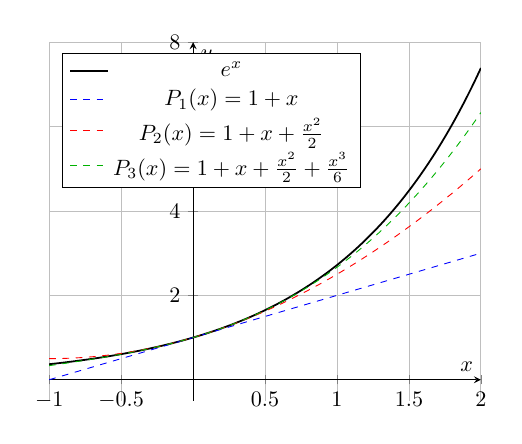
\begin{tikzpicture}[scale=0.8]
\begin{axis}[
    axis lines=middle,
    xlabel={$x$},
    ylabel={$y$},
    domain=-1:2,
    samples=100,
    grid=major,
    legend pos=north west,
    ymin=-0.5, ymax=8
]
\addplot[black, thick] {exp(x)};
\addlegendentry{$e^x$}

\addplot[blue, dashed] {1 + x};
\addlegendentry{$P_1(x) = 1 + x$}

\addplot[red, dashed] {1 + x + x^2/2};
\addlegendentry{$P_2(x) = 1 + x + \frac{x^2}{2}$}

\addplot[green!70!black, dashed] {1 + x + x^2/2 + x^3/6};
\addlegendentry{$P_3(x) = 1 + x + \frac{x^2}{2} + \frac{x^3}{6}$}
\end{axis}
\end{tikzpicture}
\end{center}
Higher-degree polynomials provide better approximations near $x = 0$.
\end{frame}

\begin{frame}{Taylor's Theorem with Remainder}
\textbf{Taylor's Theorem:} If $f$ has $n+1$ continuous derivatives, then:
$$f(x) = P_n(x) + R_n(x)$$

where $P_n(x)$ is the Taylor polynomial and $R_n(x)$ is the remainder term.

\vspace{0.5cm}

\textbf{Lagrange Form of Remainder:}
$$R_n(x) = \frac{f^{(n+1)}(c)}{(n+1)!}(x-a)^{n+1}$$

for some $c$ between $a$ and $x$.

\vspace{0.5cm}

This tells us the \textit{error} in approximating $f(x)$ by $P_n(x)$.
\end{frame}

\section{Concave and Convex Functions}

\begin{frame}{Definition of Convexity}
A function $f$ is \textbf{convex} on an interval $I$ if for all $x_1, x_2 \in I$ and $\lambda \in [0,1]$:
$$f(\lambda x_1 + (1-\lambda) x_2) \leq \lambda f(x_1) + (1-\lambda) f(x_2)$$

\vspace{0.5cm}

\textbf{Geometric Interpretation:} The line segment connecting any two points on the graph lies \textit{above} the graph.

\vspace{0.5cm}

A function $f$ is \textbf{concave} if $-f$ is convex, or equivalently:
$$f(\lambda x_1 + (1-\lambda) x_2) \geq \lambda f(x_1) + (1-\lambda) f(x_2)$$

\vspace{0.3cm}

The line segment lies \textit{below} the graph.
\end{frame}

\begin{frame}{Visualizing Convex and Concave Functions}
\begin{center}
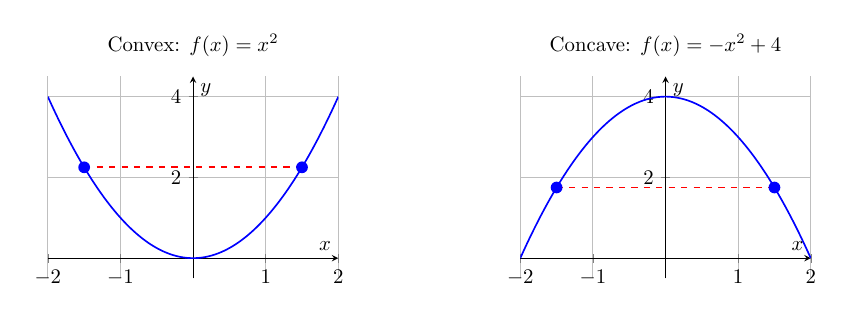
\begin{tikzpicture}[scale=0.75]
% Convex function
\begin{scope}[xshift=0cm]
\begin{axis}[
    axis lines=middle,
    xlabel={$x$},
    ylabel={$y$},
    title={Convex: $f(x) = x^2$},
    domain=-2:2,
    samples=100,
    grid=major,
    ymin=-0.5, ymax=4.5,
    width=6.5cm,
    height=5cm
]
\addplot[blue, thick] {x^2};
\addplot[red, dashed, thick] coordinates {(-1.5, 2.25) (1.5, 2.25)};
\node[circle, fill=blue, inner sep=2pt] at (axis cs:-1.5,2.25) {};
\node[circle, fill=blue, inner sep=2pt] at (axis cs:1.5,2.25) {};
\end{axis}
\end{scope}

% Concave function
\begin{scope}[xshift=8cm]
\begin{axis}[
    axis lines=middle,
    xlabel={$x$},
    ylabel={$y$},
    title={Concave: $f(x) = -x^2 + 4$},
    domain=-2:2,
    samples=100,
    grid=major,
    ymin=-0.5, ymax=4.5,
    width=6.5cm,
    height=5cm
]
\addplot[blue, thick] {-x^2 + 4};
\addplot[red, dashed, thick] coordinates {(-1.5, 1.75) (1.5, 1.75)};
\node[circle, fill=blue, inner sep=2pt] at (axis cs:-1.5,1.75) {};
\node[circle, fill=blue, inner sep=2pt] at (axis cs:1.5,1.75) {};
\end{axis}
\end{scope}
\end{tikzpicture}
\end{center}
\end{frame}

\begin{frame}{Second Derivative Test for Convexity}
\textbf{Theorem:} Let $f$ be twice differentiable on an interval $I$.

\vspace{0.5cm}

\begin{itemize}
    \item If $f''(x) \geq 0$ for all $x \in I$, then $f$ is \textbf{convex} on $I$
    \vspace{0.3cm}
    \item If $f''(x) \leq 0$ for all $x \in I$, then $f$ is \textbf{concave} on $I$
    \vspace{0.3cm}
    \item If $f''(x) > 0$ for all $x \in I$, then $f$ is \textbf{strictly convex} on $I$
    \vspace{0.3cm}
    \item If $f''(x) < 0$ for all $x \in I$, then $f$ is \textbf{strictly concave} on $I$
\end{itemize}

\vspace{0.5cm}

\textbf{Intuition:} 
\begin{itemize}
    \item $f''(x) > 0$: function curves upward (convex, "holds water")
    \item $f''(x) < 0$: function curves downward (concave, "spills water")
\end{itemize}
\end{frame}

\begin{frame}{Examples of Convex and Concave Functions}
\textbf{Convex Functions:}
\begin{itemize}
    \item $f(x) = x^2$ \quad ($f''(x) = 2 > 0$)
    \item $f(x) = e^x$ \quad ($f''(x) = e^x > 0$)
    \item $f(x) = |x|$ \quad (convex but not differentiable at $x=0$)
    \item $f(x) = -\ln(x)$ for $x > 0$ \quad ($f''(x) = \frac{1}{x^2} > 0$)
\end{itemize}

\vspace{0.5cm}

\textbf{Concave Functions:}
\begin{itemize}
    \item $f(x) = -x^2$ \quad ($f''(x) = -2 < 0$)
    \item $f(x) = \ln(x)$ for $x > 0$ \quad ($f''(x) = -\frac{1}{x^2} < 0$)
    \item $f(x) = \sqrt{x}$ for $x \geq 0$ \quad ($f''(x) = -\frac{1}{4x^{3/2}} < 0$ for $x > 0$)
\end{itemize}
\end{frame}

\begin{frame}{Inflection Points}
\textbf{Definition:} A point $(c, f(c))$ is an \textbf{inflection point} if:
\begin{itemize}
    \item $f''(c) = 0$ or $f''(c)$ does not exist, AND
    \item $f''$ changes sign at $x = c$
\end{itemize}

\vspace{0.5cm}

At an inflection point, the function changes from convex to concave (or vice versa).

\vspace{0.5cm}

\textbf{Example:} $f(x) = x^3$
\begin{itemize}
    \item $f'(x) = 3x^2$
    \item $f''(x) = 6x$
    \item $f''(0) = 0$
    \item $f''(x) < 0$ for $x < 0$ (concave)
    \item $f''(x) > 0$ for $x > 0$ (convex)
    \item Inflection point at $(0, 0)$
\end{itemize}
\end{frame}

\begin{frame}{Visualizing Inflection Points}
\begin{center}
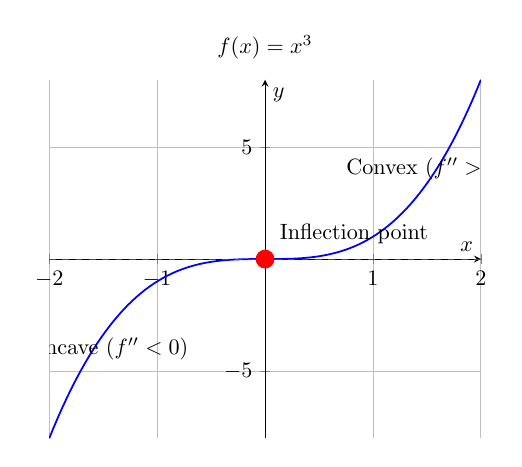
\begin{tikzpicture}[scale=0.8]
\begin{axis}[
    axis lines=middle,
    xlabel={$x$},
    ylabel={$y$},
    domain=-2:2,
    samples=100,
    grid=major,
    ymin=-8, ymax=8,
    title={$f(x) = x^3$}
]
\addplot[blue, thick] {x^3};
\node[circle, fill=red, inner sep=3pt, label=above right:{Inflection point}] at (axis cs:0,0) {};

% Add tangent line at inflection point
\addplot[red, dashed] {0};

% Annotations
\node at (axis cs:-1.5,-4) {Concave ($f'' < 0$)};
\node at (axis cs:1.5,4) {Convex ($f'' > 0$)};
\end{axis}
\end{tikzpicture}
\end{center}
\end{frame}

\section{First and Second Derivative Tests}

\begin{frame}{Critical Points}
\textbf{Definition:} A point $x = c$ is a \textbf{critical point} of $f$ if:
\begin{itemize}
    \item $f'(c) = 0$, OR
    \item $f'(c)$ does not exist
\end{itemize}

\vspace{0.5cm}

\textbf{Why are critical points important?}
\begin{itemize}
    \item Local maxima and minima occur at critical points
    \item Not all critical points are local extrema (e.g., inflection points)
\end{itemize}

\vspace{0.5cm}

\textbf{Example:} $f(x) = x^3 - 3x^2 + 2$
\begin{itemize}
    \item $f'(x) = 3x^2 - 6x = 3x(x-2)$
    \item Critical points: $x = 0$ and $x = 2$
\end{itemize}
\end{frame}

\begin{frame}{First Derivative Test}
\textbf{First Derivative Test:} Let $c$ be a critical point of $f$.

\vspace{0.5cm}

\textbf{Local Maximum at $x = c$:}
\begin{itemize}
    \item $f'(x) > 0$ for $x < c$ (increasing)
    \item $f'(x) < 0$ for $x > c$ (decreasing)
\end{itemize}

\vspace{0.3cm}

\textbf{Local Minimum at $x = c$:}
\begin{itemize}
    \item $f'(x) < 0$ for $x < c$ (decreasing)
    \item $f'(x) > 0$ for $x > c$ (increasing)
\end{itemize}

\vspace{0.3cm}

\textbf{Neither (possible inflection point):}
\begin{itemize}
    \item $f'$ does not change sign at $x = c$
\end{itemize}

\vspace{0.3cm}

\textbf{Summary:} Look at the \textit{sign change} of $f'(x)$ around $x = c$.
\end{frame}

\begin{frame}{Visualizing the First Derivative Test}
\begin{center}
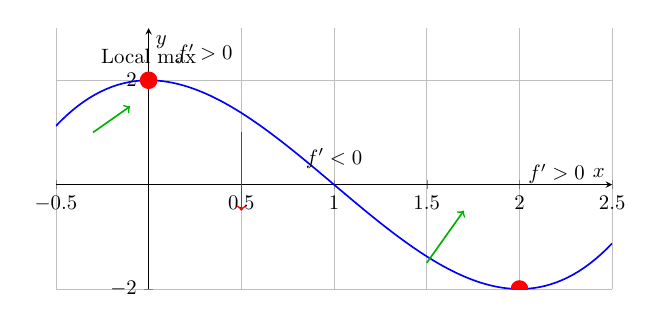
\begin{tikzpicture}[scale=0.75]
\begin{axis}[
    axis lines=middle,
    xlabel={$x$},
    ylabel={$y$},
    domain=-0.5:2.5,
    samples=100,
    grid=major,
    ymin=-2, ymax=3,
    width=11cm,
    height=6cm
]
\addplot[blue, thick] {x^3 - 3*x^2 + 2};

% Mark critical points
\node[circle, fill=red, inner sep=3pt, label=above:{Local max}] at (axis cs:0,2) {};
\node[circle, fill=red, inner sep=3pt, label=below:{Local min}] at (axis cs:2,-2) {};

% Add arrows to show behavior
\draw[->, thick, green!70!black] (axis cs:-0.3,1) -- (axis cs:-0.1,1.5);
\draw[->, thick, red] (axis cs:0.5,1) -- (axis cs:0.5,-0.5);
\draw[->, thick, green!70!black] (axis cs:1.5,-1.5) -- (axis cs:1.7,-0.5);

\node at (axis cs:0.3, 2.5) {$f' > 0$};
\node at (axis cs:1, 0.5) {$f' < 0$};
\node at (axis cs:2.2, 0.2) {$f' > 0$};
\end{axis}
\end{tikzpicture}
\end{center}
\end{frame}

\begin{frame}{Second Derivative Test}
\textbf{Second Derivative Test:} Let $c$ be a critical point with $f'(c) = 0$.

\vspace{0.5cm}

\begin{itemize}
    \item If $f''(c) > 0$, then $f$ has a \textbf{local minimum} at $x = c$
    
    \vspace{0.2cm}
    (function is convex near $c$, curves upward)
    
    \vspace{0.5cm}
    
    \item If $f''(c) < 0$, then $f$ has a \textbf{local maximum} at $x = c$
    
    \vspace{0.2cm}
    (function is concave near $c$, curves downward)
    
    \vspace{0.5cm}
    
    \item If $f''(c) = 0$, the test is \textbf{inconclusive}
    
    \vspace{0.2cm}
    (use first derivative test or higher-order derivatives)
\end{itemize}

\vspace{0.5cm}

\textbf{Advantage:} Only need to evaluate $f''$ at the critical point, not in an interval.
\end{frame}

\begin{frame}{Example: Finding Local Extrema}
\textbf{Find and classify the critical points of} $f(x) = x^3 - 3x^2 + 2$

\vspace{0.3cm}

\textbf{Step 1: Find critical points}
$$f'(x) = 3x^2 - 6x = 3x(x-2) = 0$$
Critical points: $x = 0$ and $x = 2$

\vspace{0.3cm}

\textbf{Step 2: Apply second derivative test}
$$f''(x) = 6x - 6$$

At $x = 0$: $f''(0) = -6 < 0$ $\Rightarrow$ \textbf{local maximum}

$f(0) = 2$, so local maximum at $(0, 2)$

\vspace{0.3cm}

At $x = 2$: $f''(2) = 6 > 0$ $\Rightarrow$ \textbf{local minimum}

$f(2) = -2$, so local minimum at $(2, -2)$
\end{frame}

\begin{frame}{Comparison: First vs. Second Derivative Test}
\begin{center}
\begin{tabular}{|p{5.5cm}|p{5.5cm}|}
\hline
\textbf{First Derivative Test} & \textbf{Second Derivative Test} \\
\hline
Requires checking sign of $f'$ on both sides of critical point & Only requires evaluating $f''$ at the critical point \\
\hline
Always works (assuming $f'$ exists) & May be inconclusive if $f''(c) = 0$ \\
\hline
More information about behavior & Less information, but faster \\
\hline
\end{tabular}
\end{center}

\vspace{0.5cm}

\textbf{When to use which test?}
\begin{itemize}
    \item Use \textbf{second derivative test} if it's easy to compute $f''(c)$ and $f''(c) \neq 0$
    \item Use \textbf{first derivative test} if second derivative test is inconclusive or complicated
\end{itemize}
\end{frame}

\begin{frame}{Example Where Second Derivative Test Fails}
\textbf{Example:} $f(x) = x^4$

\vspace{0.3cm}

$f'(x) = 4x^3 = 0$ at $x = 0$ (critical point)

$f''(x) = 12x^2$, so $f''(0) = 0$ (inconclusive!)

\vspace{0.5cm}

\textbf{Use first derivative test:}
\begin{itemize}
    \item For $x < 0$: $f'(x) = 4x^3 < 0$ (decreasing)
    \item For $x > 0$: $f'(x) = 4x^3 > 0$ (increasing)
\end{itemize}

Therefore, $f$ has a \textbf{local minimum} at $x = 0$.

\vspace{0.5cm}

\textbf{Alternative:} Check $f'''(0) = 0$ and $f^{(4)}(0) = 24 > 0$

Higher-order derivative tests exist, but are rarely used.
\end{frame}

\begin{frame}{Visualizing Local Extrema with Derivatives}
\begin{center}
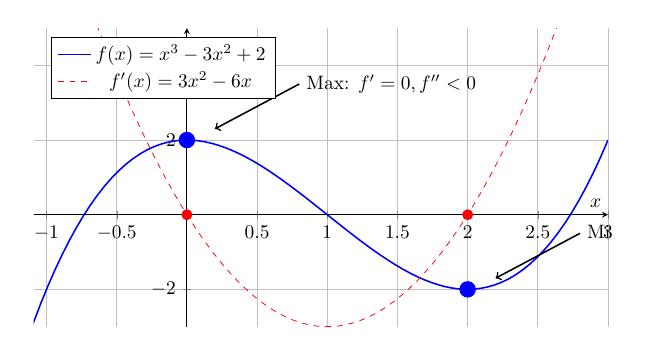
\begin{tikzpicture}[scale=0.7]
\begin{axis}[
    axis lines=middle,
    xlabel={$x$},
    ylabel={},
    domain=-2:3,
    samples=100,
    grid=major,
    ymin=-3, ymax=5,
    width=12cm,
    height=7cm,
    legend pos=north west
]
% Function
\addplot[blue, thick] {x^3 - 3*x^2 + 2};
\addlegendentry{$f(x) = x^3 - 3x^2 + 2$}

% First derivative
\addplot[red, dashed] {3*x^2 - 6*x};
\addlegendentry{$f'(x) = 3x^2 - 6x$}

% Mark where f' = 0
\node[circle, fill=red, inner sep=2pt] at (axis cs:0,0) {};
\node[circle, fill=red, inner sep=2pt] at (axis cs:2,0) {};

% Mark extrema on f
\node[circle, fill=blue, inner sep=3pt] at (axis cs:0,2) {};
\node[circle, fill=blue, inner sep=3pt] at (axis cs:2,-2) {};

\draw[<-, thick] (axis cs:0.2,2.3) -- (axis cs:0.8,3.5) node[right] {Max: $f'=0, f''<0$};
\draw[<-, thick] (axis cs:2.2,-1.7) -- (axis cs:2.8,-0.5) node[right] {Min: $f'=0, f''>0$};
\end{axis}
\end{tikzpicture}
\end{center}
\end{frame}

\begin{frame}{Summary}
\textbf{Higher-Order Derivatives:}
\begin{itemize}
    \item Provide information about curvature and behavior
    \item Physical interpretation: velocity, acceleration, jerk
\end{itemize}

\vspace{0.3cm}

\textbf{Taylor's Theorem:}
\begin{itemize}
    \item Approximates functions with polynomials
    \item Better approximation with more terms
\end{itemize}

\vspace{0.3cm}

\textbf{Convexity and Concavity:}
\begin{itemize}
    \item $f''(x) > 0 \Rightarrow$ convex (curves up)
    \item $f''(x) < 0 \Rightarrow$ concave (curves down)
    \item Inflection points where $f''$ changes sign
\end{itemize}

\vspace{0.3cm}

\textbf{Derivative Tests:}
\begin{itemize}
    \item First derivative test: check sign change of $f'$
    \item Second derivative test: check sign of $f''$ at critical point
\end{itemize}
\end{frame}

\begin{frame}{Practice Problems}
\textbf{Problem 1:} Find the Taylor polynomial of degree 3 for $f(x) = \cos(x)$ at $x = 0$.

\vspace{0.5cm}

\textbf{Problem 2:} Determine where $f(x) = x^4 - 4x^3$ is convex and concave.

\vspace{0.5cm}

\textbf{Problem 3:} Find and classify all critical points of $f(x) = x^3 - 6x^2 + 9x + 1$ using both the first and second derivative tests.

\vspace{0.5cm}

\textbf{Problem 4:} Find the inflection points of $f(x) = x^4 - 6x^2 + 8x - 3$.
\end{frame}

\end{document}
